\begin{figure}
\centering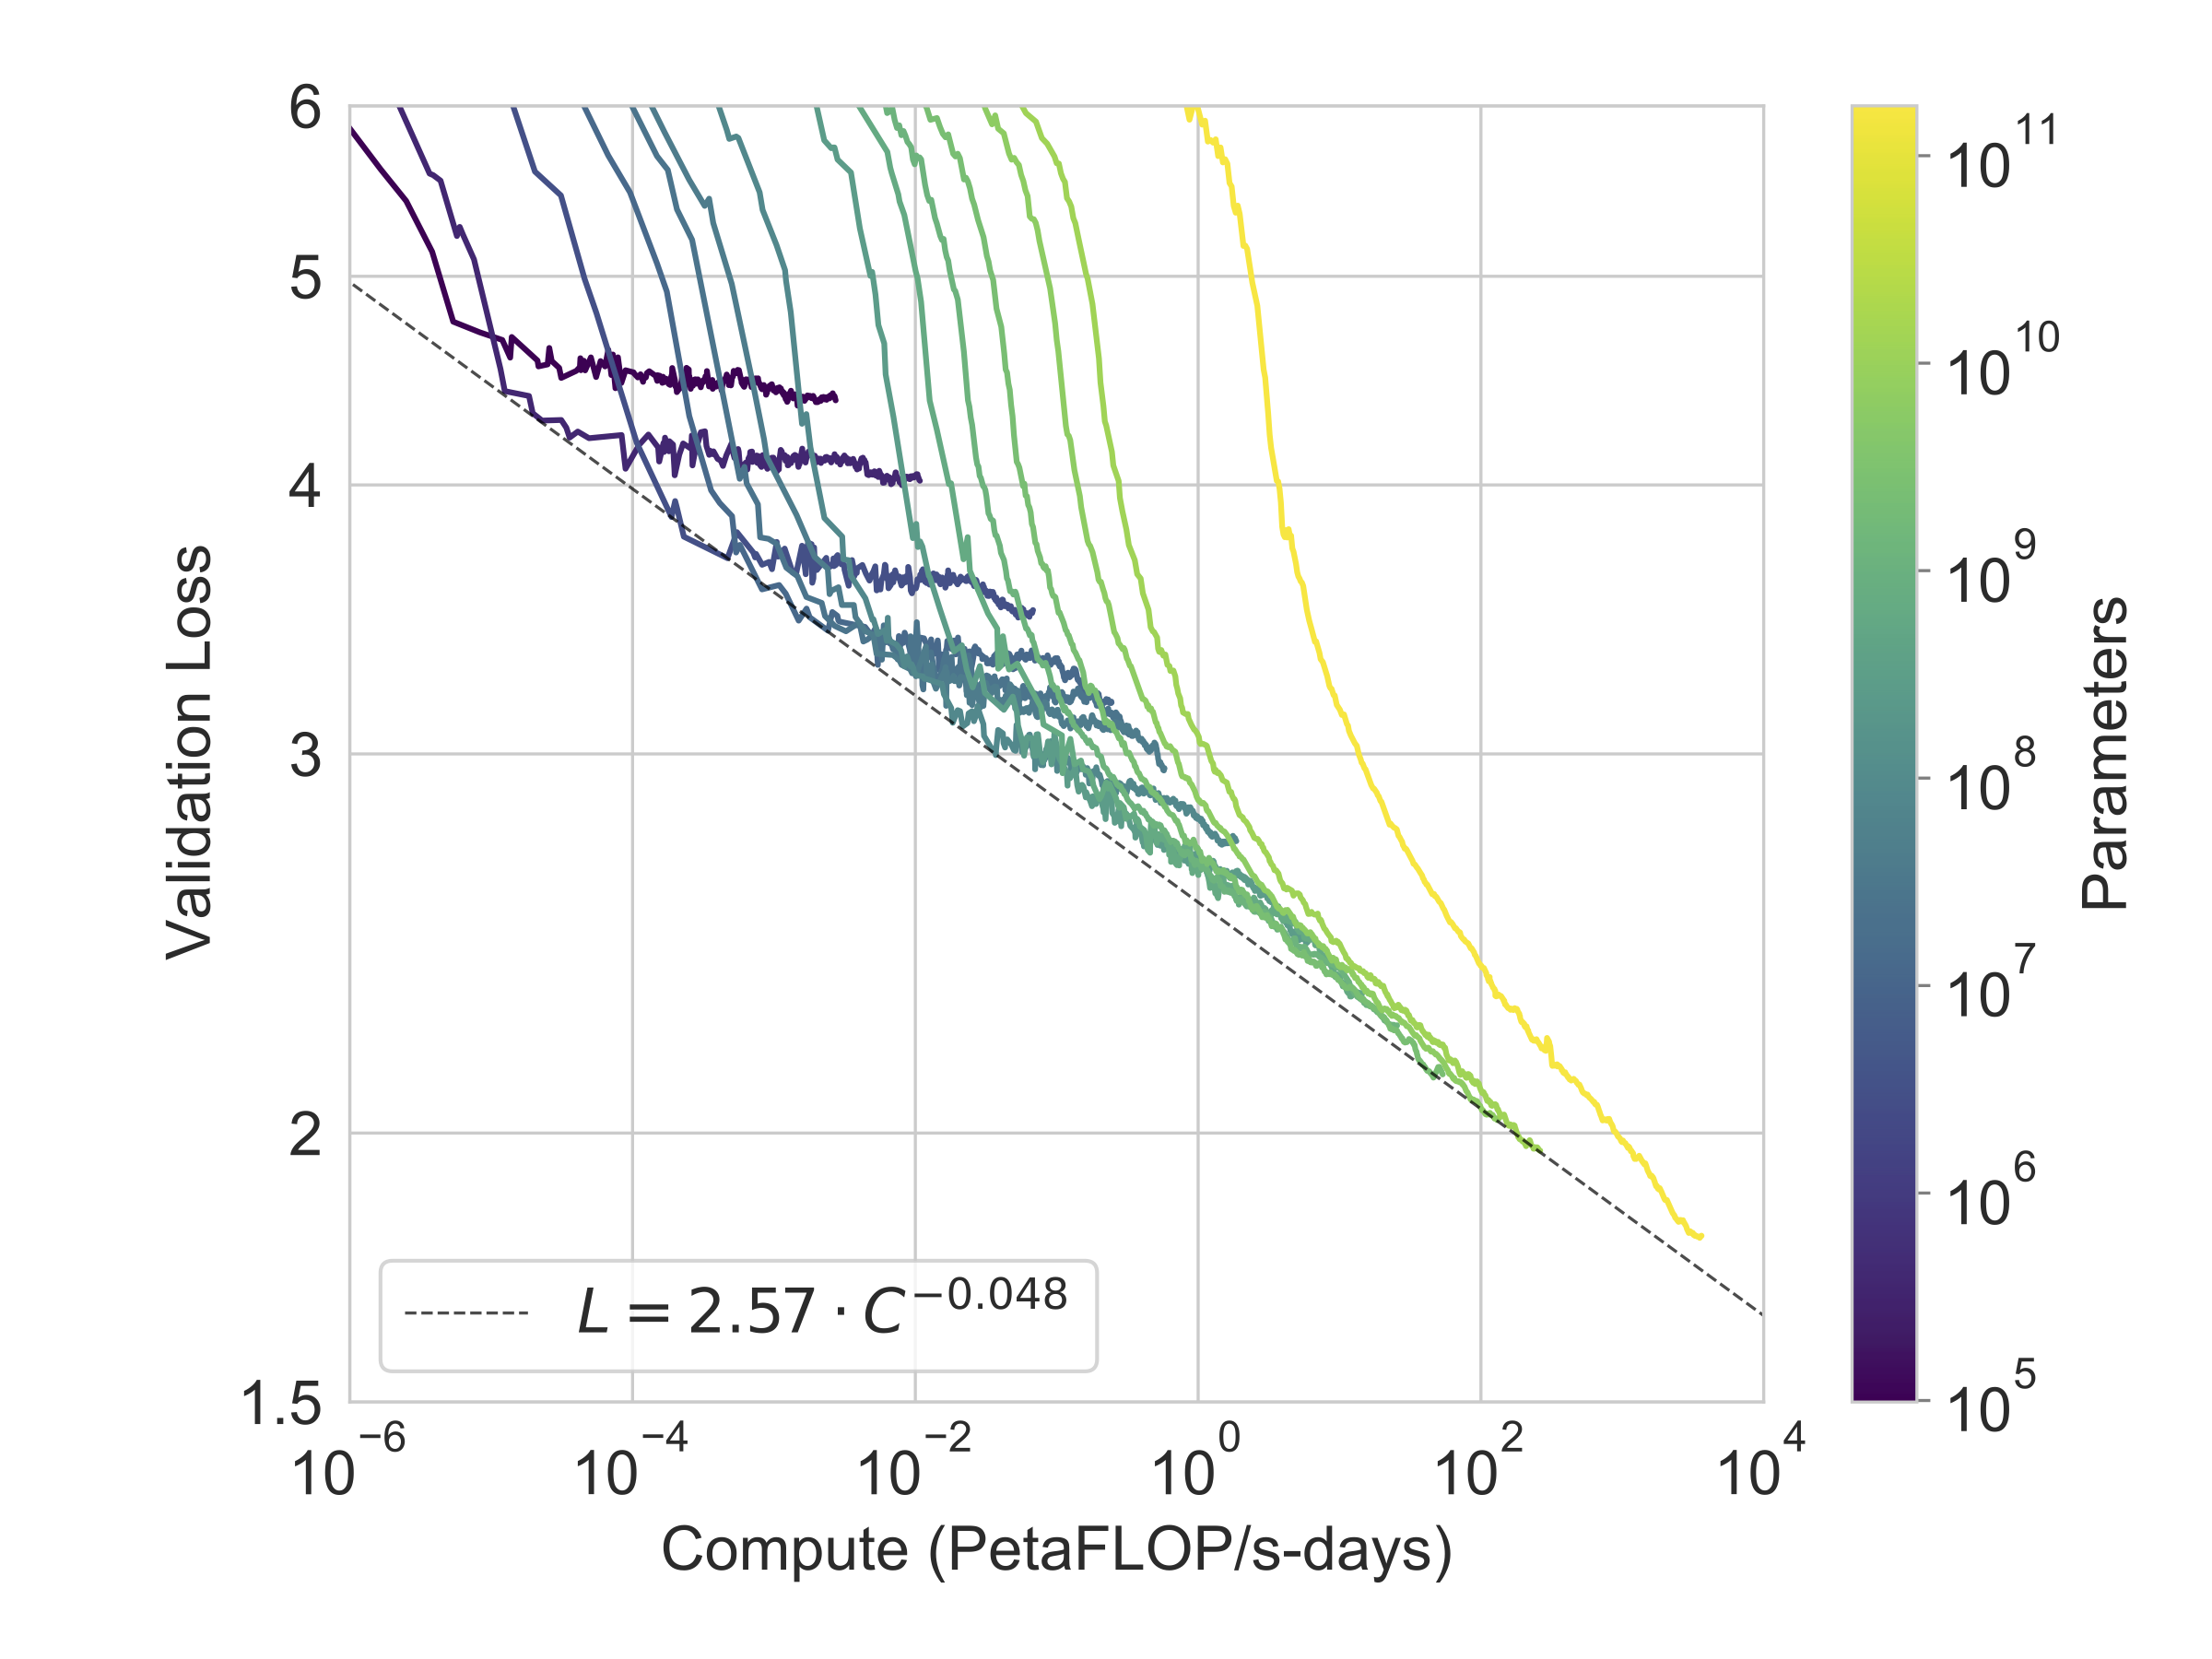
\includegraphics[width=0.7\linewidth]{graphs/img/LanguageModelingComputePareto.png}
\caption{\textbf{Smooth scaling of performance with compute.} Performance (measured in terms of cross-entropy validation loss) follows a power-law trend with the amount of compute used for training. The power-law behavior observed in \cite{kaplan2020scaling} continues for an additional two orders of magnitude with only small deviations from the predicted curve.  For this figure, we exclude embedding parameters from compute and parameter counts.}
\label{graph:compute}
\end{figure}